% Options for packages loaded elsewhere
\PassOptionsToPackage{unicode}{hyperref}
\PassOptionsToPackage{hyphens}{url}
\documentclass[
  ignorenonframetext,
]{beamer}
\newif\ifbibliography
\usepackage{pgfpages}
\setbeamertemplate{caption}[numbered]
\setbeamertemplate{caption label separator}{: }
\setbeamercolor{caption name}{fg=normal text.fg}
\beamertemplatenavigationsymbolsempty
% remove section numbering
\setbeamertemplate{part page}{
  \centering
  \begin{beamercolorbox}[sep=16pt,center]{part title}
    \usebeamerfont{part title}\insertpart\par
  \end{beamercolorbox}
}
\setbeamertemplate{section page}{
  \centering
  \begin{beamercolorbox}[sep=12pt,center]{section title}
    \usebeamerfont{section title}\insertsection\par
  \end{beamercolorbox}
}
\setbeamertemplate{subsection page}{
  \centering
  \begin{beamercolorbox}[sep=8pt,center]{subsection title}
    \usebeamerfont{subsection title}\insertsubsection\par
  \end{beamercolorbox}
}
% Prevent slide breaks in the middle of a paragraph
\widowpenalties 1 10000
\raggedbottom
\AtBeginPart{
  \frame{\partpage}
}
\AtBeginSection{
  \ifbibliography
  \else
    \frame{\sectionpage}
  \fi
}
\AtBeginSubsection{
  \frame{\subsectionpage}
}
\usepackage{iftex}
\ifPDFTeX
  \usepackage[T1]{fontenc}
  \usepackage[utf8]{inputenc}
  \usepackage{textcomp} % provide euro and other symbols
\else % if luatex or xetex
  \usepackage{unicode-math} % this also loads fontspec
  \defaultfontfeatures{Scale=MatchLowercase}
  \defaultfontfeatures[\rmfamily]{Ligatures=TeX,Scale=1}
\fi
\usepackage{lmodern}
\ifPDFTeX\else
  % xetex/luatex font selection
\fi
% Use upquote if available, for straight quotes in verbatim environments
\IfFileExists{upquote.sty}{\usepackage{upquote}}{}
\IfFileExists{microtype.sty}{% use microtype if available
  \usepackage[]{microtype}
  \UseMicrotypeSet[protrusion]{basicmath} % disable protrusion for tt fonts
}{}
\makeatletter
\@ifundefined{KOMAClassName}{% if non-KOMA class
  \IfFileExists{parskip.sty}{%
    \usepackage{parskip}
  }{% else
    \setlength{\parindent}{0pt}
    \setlength{\parskip}{6pt plus 2pt minus 1pt}}
}{% if KOMA class
  \KOMAoptions{parskip=half}}
\makeatother
\usepackage{longtable,booktabs,array}
\usepackage{caption}
\captionsetup[table]{skip=6pt}
\newcounter{none} % for unnumbered tables
\usepackage{calc} % for calculating minipage widths
\usepackage{caption}
% Make caption package work with longtable
\makeatletter
\def\fnum@table{\tablename~\thetable}
\makeatother
\usepackage{graphicx}
\makeatletter
\newsavebox\pandoc@box
\newcommand*\pandocbounded[1]{% scales image to fit in text height/width
  \sbox\pandoc@box{#1}%
  \Gscale@div\@tempa{\textheight}{\dimexpr\ht\pandoc@box+\dp\pandoc@box\relax}%
  \Gscale@div\@tempb{\linewidth}{\wd\pandoc@box}%
  \ifdim\@tempb\p@<\@tempa\p@\let\@tempa\@tempb\fi% select the smaller of both
  \ifdim\@tempa\p@<\p@\scalebox{\@tempa}{\usebox\pandoc@box}%
  \else\usebox{\pandoc@box}%
  \fi%
}
% Set default figure placement to htbp
\def\fps@figure{htbp}
\makeatother
\setlength{\emergencystretch}{3em} % prevent overfull lines
\providecommand{\tightlist}{%
  \setlength{\itemsep}{0pt}\setlength{\parskip}{0pt}}
% Manuscript macro/package fallbacks (newcommand -> providecommand).
\usepackage{amsmath}
\usepackage{amssymb}
\usepackage{booktabs}

% Slide layout defaults for warning-clean scientific decks.
\usepackage{etoolbox}
\IfFileExists{xurl.sty}{\usepackage{xurl}}{}
\IfFileExists{seqsplit.sty}{\usepackage{seqsplit}}{\newcommand{\seqsplit}[1]{#1}}
\protected\def\breakseq#1{\seqsplit{#1}}
\protected\def\breaktt#1{\begingroup\ttfamily\seqsplit{#1}\endgroup}
\setlength{\emergencystretch}{6em}
\tolerance=5000
\hbadness=10000
\hfuzz=1pt
\setlength{\tabcolsep}{2pt}
\AtBeginEnvironment{longtable}{\tiny\renewcommand{\arraystretch}{0.86}\setlength{\tabcolsep}{1pt}}
\AtBeginEnvironment{tabular}{\tiny\renewcommand{\arraystretch}{0.86}\setlength{\tabcolsep}{1pt}}
\AtBeginEnvironment{equation}{\tiny}
\AtBeginEnvironment{equation*}{\tiny}
\AtBeginEnvironment{align}{\tiny}
\AtBeginEnvironment{align*}{\tiny}
\AtBeginEnvironment{itemize}{\footnotesize}
\AtBeginEnvironment{enumerate}{\footnotesize}
\AtBeginEnvironment{description}{\footnotesize}
\setbeamerfont{caption}{size=\tiny}
\setbeamerfont{caption name}{size=\tiny}
\setbeamerfont{normal text}{size=\small}
\setbeamerfont{frametitle}{size=\small}
\setbeamerfont{section title}{size=\footnotesize}
\setbeamerfont{subsection title}{size=\footnotesize}
\setbeamertemplate{section page}{%
  \centering
  \begin{beamercolorbox}[sep=12pt,center,wd=\paperwidth]{section title}
    \parbox{0.86\paperwidth}{\centering\usebeamerfont{section title}\insertsection\par}
  \end{beamercolorbox}
}
\setbeamertemplate{subsection page}{%
  \centering
  \begin{beamercolorbox}[sep=8pt,center,wd=\paperwidth]{subsection title}
    \parbox{0.86\paperwidth}{\centering\usebeamerfont{subsection title}\insertsubsection\par}
  \end{beamercolorbox}
}
\setlength{\abovecaptionskip}{2pt}
\setlength{\belowcaptionskip}{0pt}

% Natbib and cross-reference fallbacks — slides don't load natbib
% or cleveref, but combined-PDF manuscript prose may emit these
% commands. The fallback renders citations as a bracketed key list
% and cross-references as detokenized labels so slides don't fail on
% undefined control sequences or raw underscores. \providecommand is
% a no-op if packages load later.
\providecommand{\citep}[1]{[#1]}
\providecommand{\citet}[1]{#1}
\providecommand{\citealp}[1]{#1}
\providecommand{\citeauthor}[1]{#1}
\providecommand{\citeyear}[1]{#1}
\providecommand{\cref}[1]{\texttt{\detokenize{#1}}}
\providecommand{\Cref}[1]{\texttt{\detokenize{#1}}}
\providecommand{\crefrange}[2]{\texttt{\detokenize{#1}}--\texttt{\detokenize{#2}}}
\providecommand{\Crefrange}[2]{\texttt{\detokenize{#1}}--\texttt{\detokenize{#2}}}
\providecommand{\paragraph}[1]{\textbf{#1}\ }

\newtheorem{proposition}{Proposition}
\newtheorem{hypothesis}{Hypothesis}
\newtheorem{remark}[theorem]{Remark}
\newtheorem{axiom}{Axiom}
\newtheorem{property}{Property}
\usepackage{bookmark}
\IfFileExists{xurl.sty}{\usepackage{xurl}}{} % add URL line breaks if available
\urlstyle{same}
% fallback for those not using the hyperref driver hyperxmp:
\makeatletter
\@ifundefined{xmpquote}{\newcommand{\xmpquote}[1]{#1}}{}
\makeatother
\hypersetup{
  hidelinks,
  pdfcreator={LaTeX via pandoc}}

\author{\texorpdfstring{}{}}
\date{}

\begin{document}

\section{Methods}\label{sec:methods}

\begin{frame}[allowframebreaks]{Methods}
The GeneralizedNotationNotation (GNN) method is realized as a sequence
of deterministic transformations that take a plain-text model
specification and carry it through parsing, validation, code generation,
execution, and reporting. The processing pipeline is organized into 25
numbered steps (steps 0--24), each implemented as a standalone module
with a single responsibility. The methods below describe the path that a
model travels from notation to executable cognitive model and back to
analyzed results. Every quantity reported in this section is produced
from the live repository rather than asserted by hand; the closing
subsection makes that contract explicit.
\end{frame}

\begin{frame}[allowframebreaks]{Parsing and Multi-Format Export}
\protect\phantomsection\label{parsing-and-multi-format-export}
The pipeline begins by ingesting GNN model files written in the
plain-text notation. Parsing (step 3) reads each specification, builds
an internal model representation, and re-emits it across a family of
structured export formats so that downstream tools, and human readers,
can consume the same model through whichever serialization they prefer.
The corpus that exercises this stage spans 29 example model files
organized into 10 curated corpora, ranging from minimal perception
fixtures used to test the parser to larger hierarchical and multi-agent
models. The presence of hierarchical fixtures should be read as a
coverage target, not as a claim that every current backend fully
executes every hierarchical formulation; scaling hierarchical active
inference remains an active research problem in its own right
(Rangarajan and Rao 2026). Treating parsing and export as a single
\end{frame}

\begin{frame}[allowframebreaks]{Parsing and Multi-Format Export}
round-trippable stage means a model authored once becomes immediately
available as a typed object, a normalized text form, and
machine-readable serializations without any manual re-encoding.
\end{frame}

\begin{frame}[allowframebreaks]{Type Checking and Validation}
\protect\phantomsection\label{type-checking-and-validation}
A model that parses is not yet a model that is well-formed. Steps 5 and
6 apply type checking and validation to confirm that the state spaces,
observation modalities, control factors, and the matrices relating them
are mutually consistent before any code is generated. This catches
dimensional mismatches and malformed factor structures at the notation
level, where the diagnostic is cheap and legible, rather than allowing
them to surface as opaque runtime errors deep inside a numerical
backend. Validation here is the gate that protects every later stage:
rendering, execution, and analysis all assume a model that has already
been certified consistent.
\end{frame}

\begin{frame}[fragile,allowframebreaks]{Rendering to Multiple Backends}
\protect\phantomsection\label{rendering-to-multiple-backends}
The central act of the ``Triple Play'' is turning a validated
specification into executable cognitive models. The rendering stage
emits backend-specific code for 9 registered target frameworks ---
PyMDP, RxInfer.jl, ActiveInference.jl, JAX, DisCoPy, PyTorch, NumPyro,
Stan, bnlearn --- so that a single GNN model can be instantiated as a
simulation in whichever computational ecosystem a researcher already
works in; coverage across the family-by-backend matrix is uneven and is
recorded explicitly (see sec.~7). Each
backend is addressed through a registry key that maps the abstract model
onto that framework's idioms for representing generative models and
performing inference. The full mapping from registry key to backend is
given below.

\end{frame}

\begin{frame}[fragile,allowframebreaks]{Rendering to Multiple Backends}
\begin{longtable}[]{@{}lll@{}}
\caption{Render targets in
\protect\breaktt{src/render/framework\_registry.py}. The \emph{Executes}
column is the registry's own \protect\breaktt{supports\_execution} flag:
a render-only backend has no Step-12
executor.}\label{tbl:backend_registry}\tabularnewline
\toprule\noalign{}
Registry key & Backend & Executes \\
\midrule\noalign{}
\endfirsthead
\toprule\noalign{}
Registry key & Backend & Executes \\
\midrule\noalign{}
\endhead
\texttt{pymdp} & PyMDP & yes \\
\texttt{rxinfer} & RxInfer.jl & yes \\
\breaktt{activeinference\_jl} & ActiveInference.jl & yes \\
\texttt{jax} & JAX & yes \\
\texttt{discopy} & DisCoPy & yes \\
\texttt{pytorch} & PyTorch & yes \\
\texttt{numpyro} & NumPyro & yes \\
\texttt{stan} & Stan & yes \\
\texttt{bnlearn} & bnlearn & render-only \\
\bottomrule\noalign{}
\end{longtable}

\end{frame}

\begin{frame}[fragile,allowframebreaks]{Rendering to Multiple Backends}
The capability surface of these backends --- which model families each
one can express and execute --- is summarized in
fig.~\ref{fig:backend_matrix}.

\end{frame}

\begin{frame}[fragile,allowframebreaks]{Rendering to Multiple Backends}
\begin{figure}
\centering
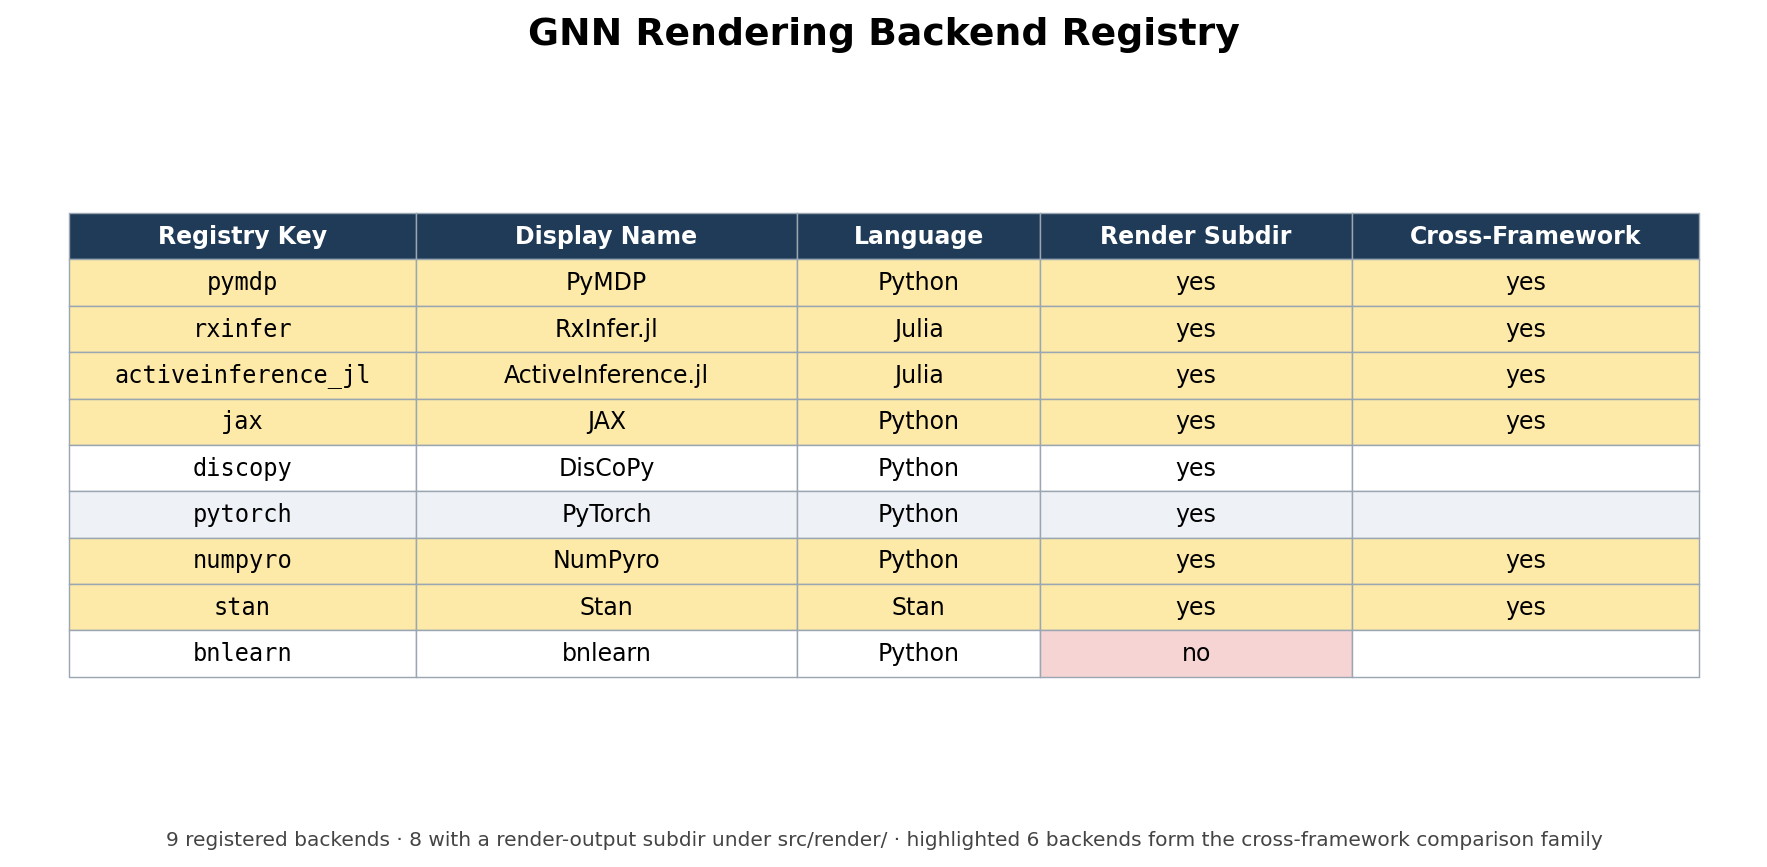
\includegraphics[width=0.85\linewidth,height=0.40\textheight,keepaspectratio,alt={The GNN rendering backend registry: each registry key, its display name, and the cross-framework comparison targets, read directly from the framework registry.}]{../figures/gnn_backend_capability_matrix.png}
\caption{The GNN rendering backend registry: each registry key, its
display name, and the cross-framework comparison targets, read directly
from the framework registry.}\label{fig:backend_matrix}
\end{figure}

\end{frame}

\begin{frame}[fragile,allowframebreaks]{Rendering to Multiple Backends}
By generating code rather than asking authors to port models by hand,
the method keeps a single source of truth in the notation while still
reaching the discrete message-passing libraries (Heins et al. 2022),
reactive message-passing lineage (Bagaev and Vries 2021), and
categorical, diagrammatic frameworks (Felice et al. 2021) that different
research communities have built. The underlying mathematics that
compatible backends share --- inference and policy selection over
discrete state spaces under the free-energy objective (Da Costa et al.
2020; Smith et al. 2022) --- is the common substrate the renderer
attempts to preserve; where a backend cannot express a family
faithfully, GNN records that boundary as an explicit unsupported status
rather than treating all registered backends as equivalent.
\end{frame}

\begin{frame}[allowframebreaks]{Execution}
\protect\phantomsection\label{execution}
Generated backend code is not left as a static artifact. The execution
stage (step 12) runs the rendered models, driving the inference and
behavior that the notation describes and producing concrete traces,
beliefs, and outputs. This closes the loop from text to running
cognitive model: the same specification that was type-checked and
exported is now exercised numerically, so that claims about a model's
behavior rest on having actually run it rather than on inspection of the
source alone.
\end{frame}

\begin{frame}[allowframebreaks]{Long-Running Orchestration Contracts}
\protect\phantomsection\label{long-running-orchestration-contracts}
GNN 3.2.0 extends the pipeline with three safe-by-design orchestration
contracts that let an extended run be observed, paused, resumed, and
audited without ever mutating live infrastructure. \emph{Durable
observation streams} record file- and array-backed stream manifests with
content checksums and replayable execution traces, so that a long run
can be re-derived deterministically before any live sensor or
device-backed stream is introduced. \emph{Resumable run sessions} carry
run-session manifests with atomic checkpoint and resume, status
inspection, and cancellation-safe cleanup, so that an extended
model-family acceptance run can be interrupted and resumed without
corrupting partial state. \emph{Auditable container plans} generate
hardened container plans together with an explicit static security
review and a rollback descriptor, deliberately stopping short of
\end{frame}

\begin{frame}[allowframebreaks]{Long-Running Orchestration Contracts}
touching any real cluster. Each contract only generates and validates
data; none performs live mutation, and each is governed by a strict
acceptance gate and exercised through dedicated Model Context Protocol
tools. fig.~\ref{fig:orchestration} shows how the three contracts
compose into one inspectable orchestration surface.

\end{frame}

\begin{frame}[allowframebreaks]{Long-Running Orchestration Contracts}
\begin{figure}
\centering
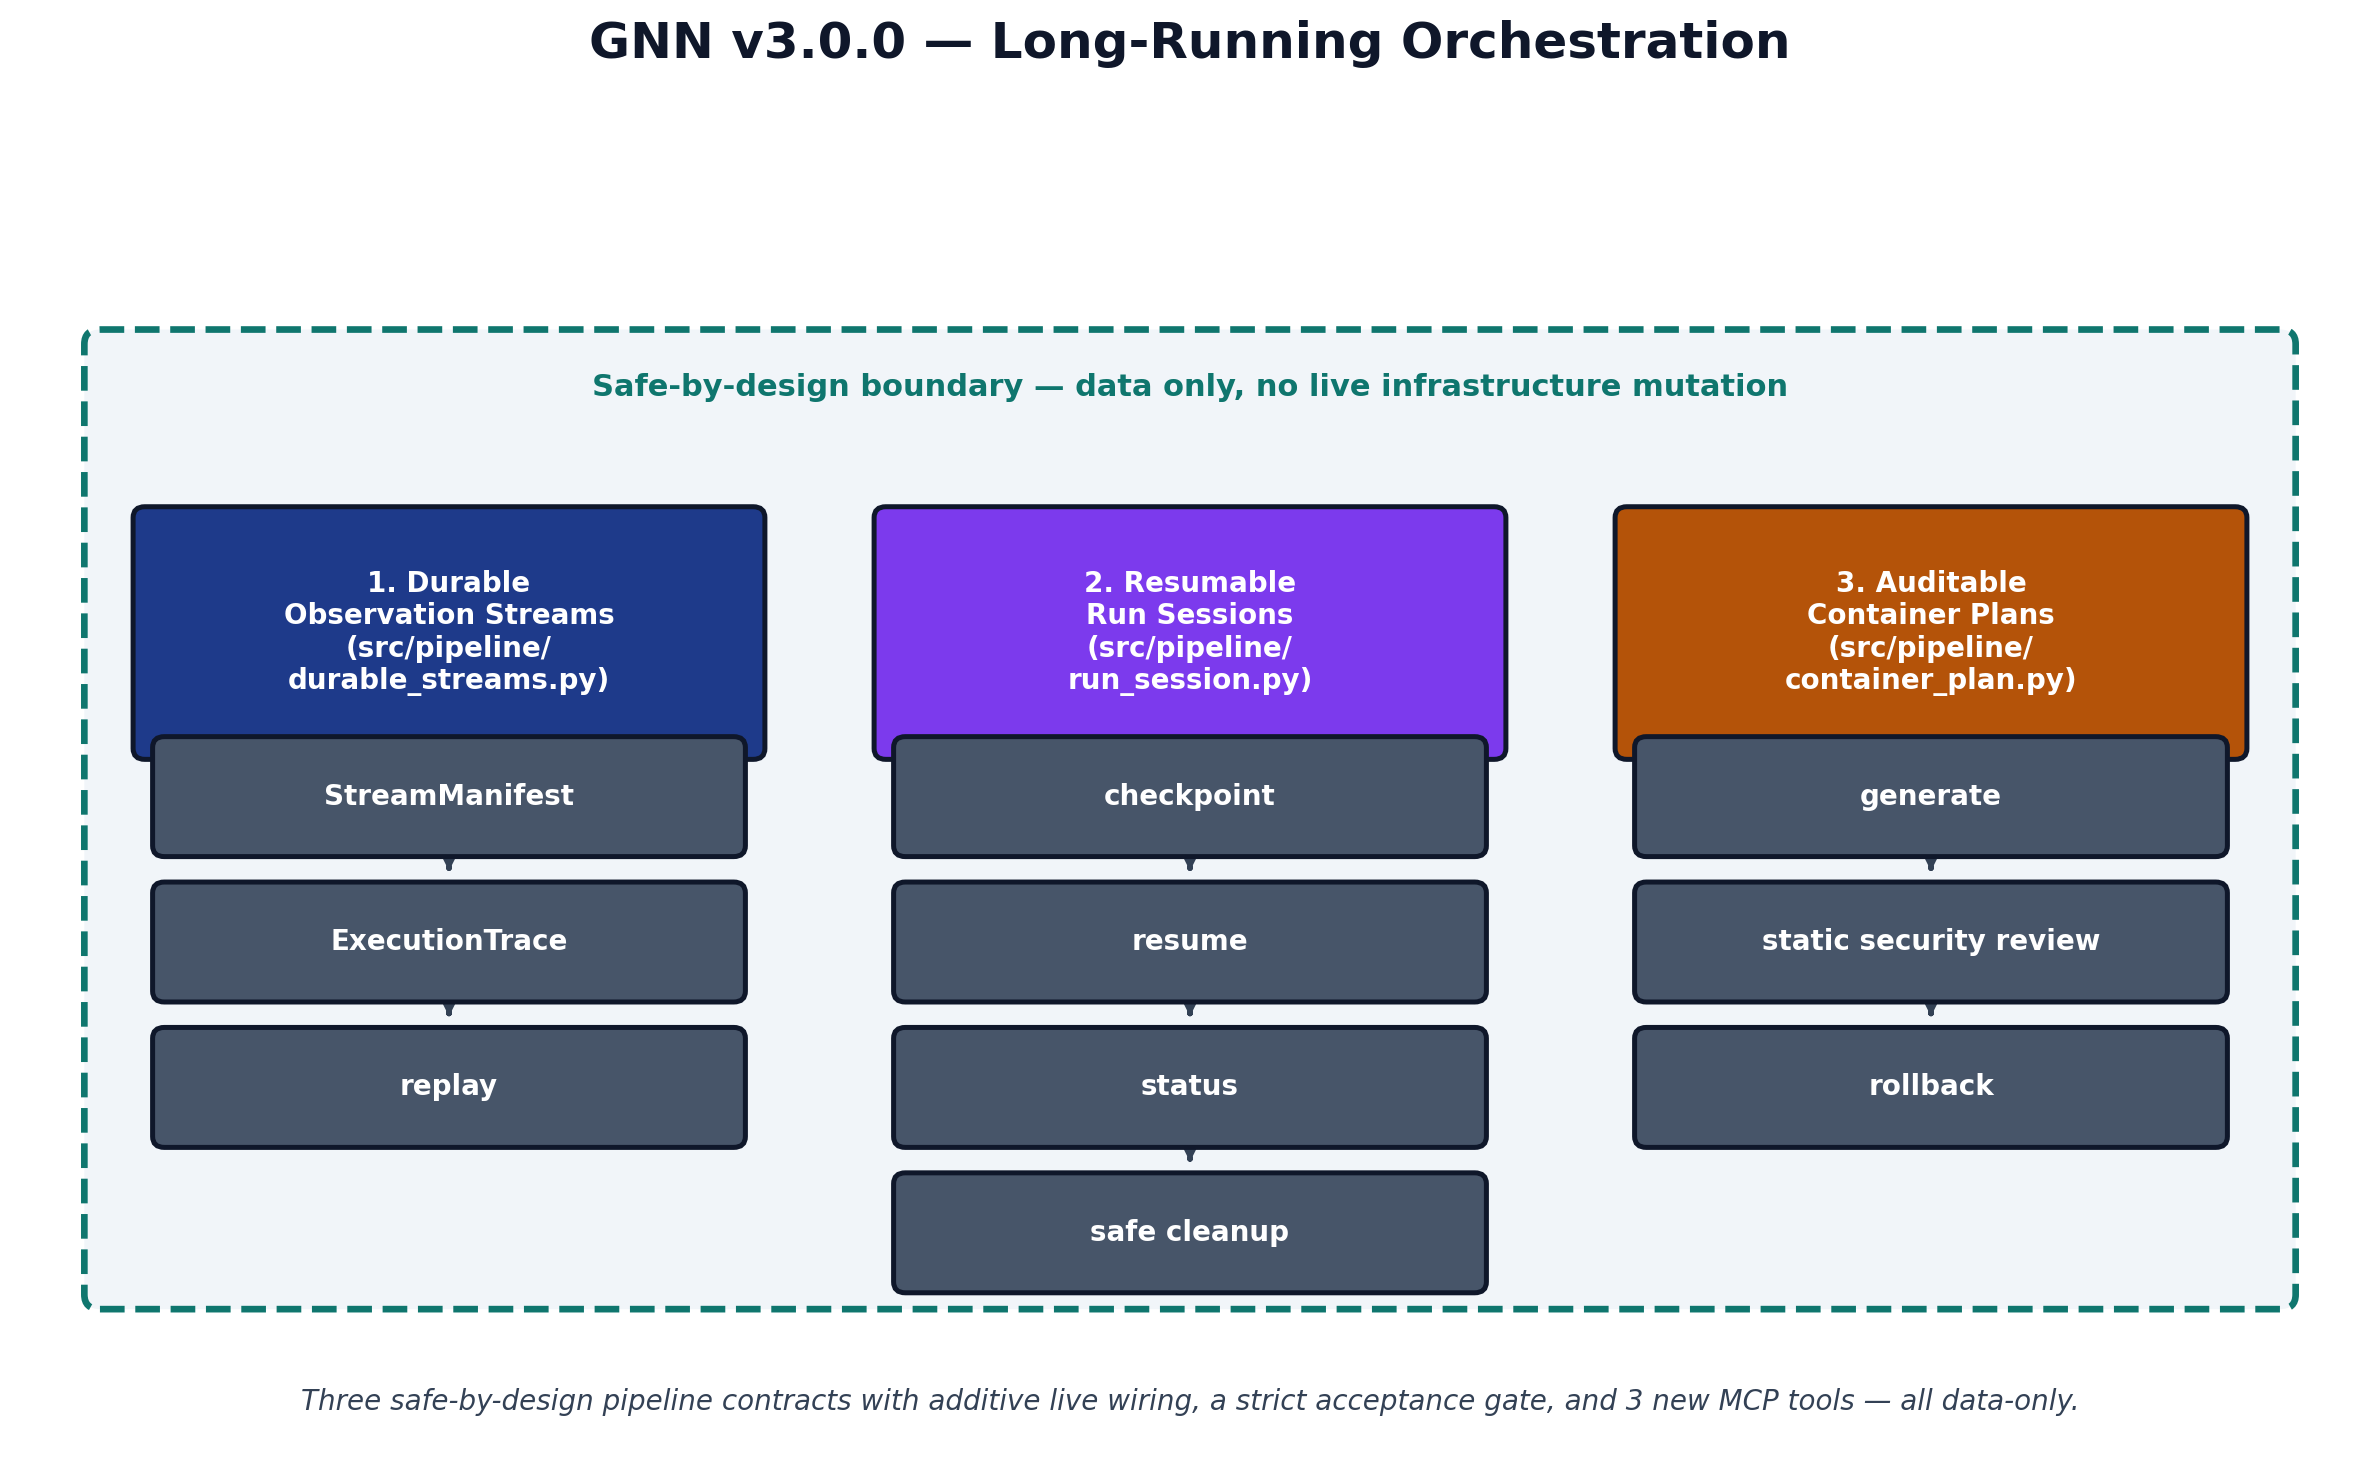
\includegraphics[width=0.85\linewidth,height=0.40\textheight,keepaspectratio,alt={The v3.0.0 long-running orchestration contracts: durable observation streams, resumable run sessions, and auditable container plans.}]{../figures/gnn_orchestration.png}
\caption{The v3.0.0 long-running orchestration contracts: durable
observation streams, resumable run sessions, and auditable container
plans.}\label{fig:orchestration}
\end{figure}
\end{frame}

\begin{frame}[allowframebreaks]{Analysis, Visualization, and Reporting}
\protect\phantomsection\label{analysis-visualization-and-reporting}
The final group of stages turns execution results into interpretable
evidence. Analysis (step 16) processes the outputs of execution into
structured findings; visualization (step 8) and the rendering of figures
(step 9) translate model structure and results into graphical form,
supporting the graphical leg of the Triple Play; and the reporting stage
(step 23) assembles these artifacts into a coherent summary of what the
model is and how it behaved. Because each stage writes its outputs to a
known location, the chain from a notation file to a finished report is
fully traceable, and any figure or number in a report can be followed
back to the step and model that produced it.
\end{frame}

\begin{frame}[fragile,allowframebreaks]{Reproducibility and
Auto-Injection}
\protect\phantomsection\label{reproducibility-and-auto-injection}
Every quantitative value that appears in this manuscript is generated,
not typed. The producer
\breaktt{scripts/z\_generate\_manuscript\_variables.py} reads the
repository's source surfaces directly --- the step modules, the source
tree, the model-family manifest, and the framework registry --- together
with the project's maintained ledgers, notably the Model Context
Protocol tool audit (\breaktt{src/mcp/audit\_report.json}, itself
regenerated by the test suite). From these it emits a manifest of named
tokens --- counts of pipeline steps, source packages and files, model
families, backends, example files, tests, and tools --- which the
renderer substitutes into the prose at build time. Filesystem-derived
counts are recomputed on every run; ledger-derived counts (such as the
MCP tool total) are as current as the ledger they read, which the
\end{frame}

\begin{frame}[fragile,allowframebreaks]{Reproducibility and
Auto-Injection}
maintained test suite keeps in sync. The manuscript therefore inherits a
determinism property: running the producer against a fixed repository
state yields the same values, and authors are prohibited from
hard-coding any number that has a corresponding token. This makes the
manuscript a faithful, regenerable description of the system it
documents: when the 25-step pipeline, the 9 rendering backends, or the
29-file example corpus change, the reported numbers change with them on
the next build, with no opportunity for prose and repository to silently
drift apart.
\end{frame}

\end{document}
